\documentclass[]{article}
\usepackage{lmodern}
\usepackage{amssymb,amsmath}
\usepackage{ifxetex,ifluatex}
\usepackage{fixltx2e} % provides \textsubscript
\ifnum 0\ifxetex 1\fi\ifluatex 1\fi=0 % if pdftex
  \usepackage[T1]{fontenc}
  \usepackage[utf8]{inputenc}
\else % if luatex or xelatex
  \ifxetex
    \usepackage{mathspec}
  \else
    \usepackage{fontspec}
  \fi
  \defaultfontfeatures{Ligatures=TeX,Scale=MatchLowercase}
\fi
% use upquote if available, for straight quotes in verbatim environments
\IfFileExists{upquote.sty}{\usepackage{upquote}}{}
% use microtype if available
\IfFileExists{microtype.sty}{%
\usepackage{microtype}
\UseMicrotypeSet[protrusion]{basicmath} % disable protrusion for tt fonts
}{}
\usepackage[margin=1in]{geometry}
\usepackage{hyperref}
\hypersetup{unicode=true,
            pdftitle={MCMC and variational bayes Representativeness, Accuracy, and Efficiency},
            pdfauthor={Ben Smith},
            pdfborder={0 0 0},
            breaklinks=true}
\urlstyle{same}  % don't use monospace font for urls
\usepackage{graphicx,grffile}
\makeatletter
\def\maxwidth{\ifdim\Gin@nat@width>\linewidth\linewidth\else\Gin@nat@width\fi}
\def\maxheight{\ifdim\Gin@nat@height>\textheight\textheight\else\Gin@nat@height\fi}
\makeatother
% Scale images if necessary, so that they will not overflow the page
% margins by default, and it is still possible to overwrite the defaults
% using explicit options in \includegraphics[width, height, ...]{}
\setkeys{Gin}{width=\maxwidth,height=\maxheight,keepaspectratio}
\IfFileExists{parskip.sty}{%
\usepackage{parskip}
}{% else
\setlength{\parindent}{0pt}
\setlength{\parskip}{6pt plus 2pt minus 1pt}
}
\setlength{\emergencystretch}{3em}  % prevent overfull lines
\providecommand{\tightlist}{%
  \setlength{\itemsep}{0pt}\setlength{\parskip}{0pt}}
\setcounter{secnumdepth}{0}
% Redefines (sub)paragraphs to behave more like sections
\ifx\paragraph\undefined\else
\let\oldparagraph\paragraph
\renewcommand{\paragraph}[1]{\oldparagraph{#1}\mbox{}}
\fi
\ifx\subparagraph\undefined\else
\let\oldsubparagraph\subparagraph
\renewcommand{\subparagraph}[1]{\oldsubparagraph{#1}\mbox{}}
\fi

%%% Use protect on footnotes to avoid problems with footnotes in titles
\let\rmarkdownfootnote\footnote%
\def\footnote{\protect\rmarkdownfootnote}

%%% Change title format to be more compact
\usepackage{titling}

% Create subtitle command for use in maketitle
\newcommand{\subtitle}[1]{
  \posttitle{
    \begin{center}\large#1\end{center}
    }
}

\setlength{\droptitle}{-2em}
  \title{MCMC and variational bayes Representativeness, Accuracy, and Efficiency}
  \pretitle{\vspace{\droptitle}\centering\huge}
  \posttitle{\par}
  \author{Ben Smith}
  \preauthor{\centering\large\emph}
  \postauthor{\par}
  \predate{\centering\large\emph}
  \postdate{\par}
  \date{9/27/2017}


\begin{document}
\maketitle

Here, I follow up the previous analysis that used Double UPdate only to
compare Variational Bayes and MCMC.

The aim is not so much to compare VB and MCMC; this has been done
adequately using MCMC. But vb takes next to no time to calculate, so we
add it in.

The information of interest is how each of the models perform in terms
of MCMC diagnostics - representativness, accuracy, and efficiency.

\section{Method}\label{method}

This time, we compare both the full, repeated-runs model as well as the
simple double-update model:

\begin{itemize}
\tightlist
\item
  \texttt{double\_update\_rpo\_repeated\_runs.stan}, the latest model
  designed for multiple runs
\item
  \texttt{double\_update.stan}, Processes only reward \emph{or}
  punishment data.
\end{itemize}

We'll run each model three times, run this for both Group 2 and Group 3,
and run on both vb and MCMC, all as for the previous comparison.
However, we will not be calculating trial posteriors, having shown how
resource intensive that is.

\begin{verbatim}
## [1] "initializing..."
\end{verbatim}

\section{Results}\label{results}

Here we are basically repeating the previous questions: how do vb and
MCMC perform in the update model with more than one run and both reward
and punishment?

\subsection{MCMC and Variational Bayes:
Reliability}\label{mcmc-and-variational-bayes-reliability}

Estimations for Punishment data appeared to differ somewhat when both
runs and when reward data was added, as we'd expect.

Is Variational bayes reliable?

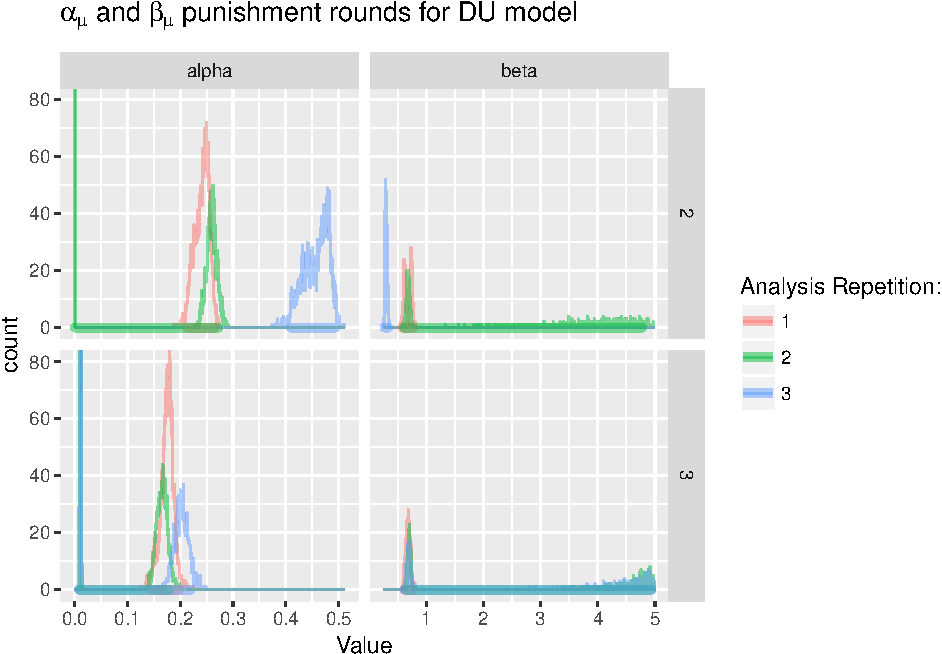
\includegraphics{compare_vb_and_MCMC_files/figure-latex/VBReliability-1.pdf}
At least using the current number of iterations and other modeling
parameters, variational bayes is not at all reliable across repeated
analyses.

How does MCMC do?

Our test is of how consistently MCMC performs across repeated analyses.

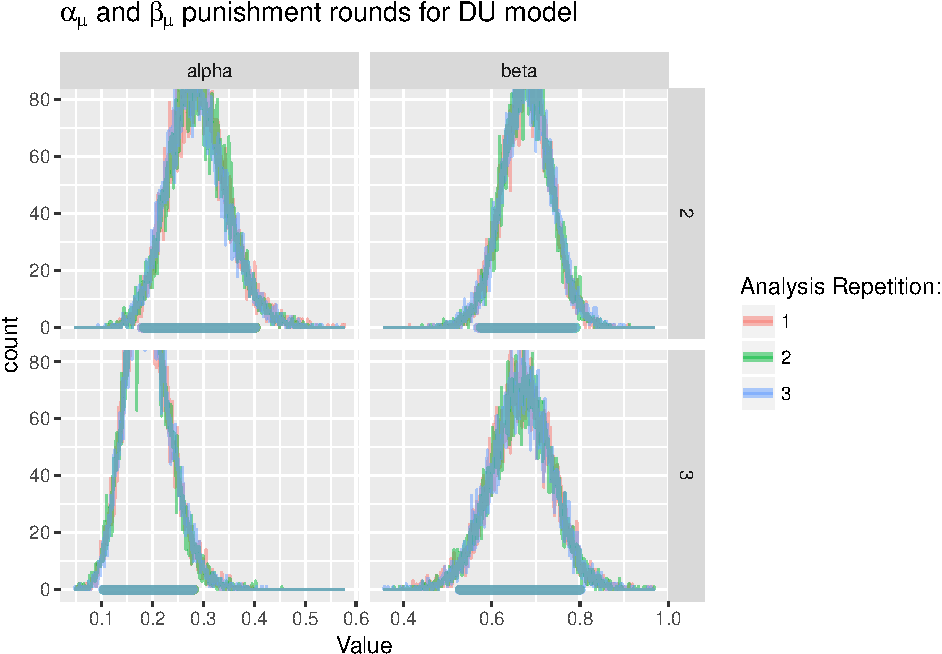
\includegraphics{compare_vb_and_MCMC_files/figure-latex/MCMCReliability-1.pdf}
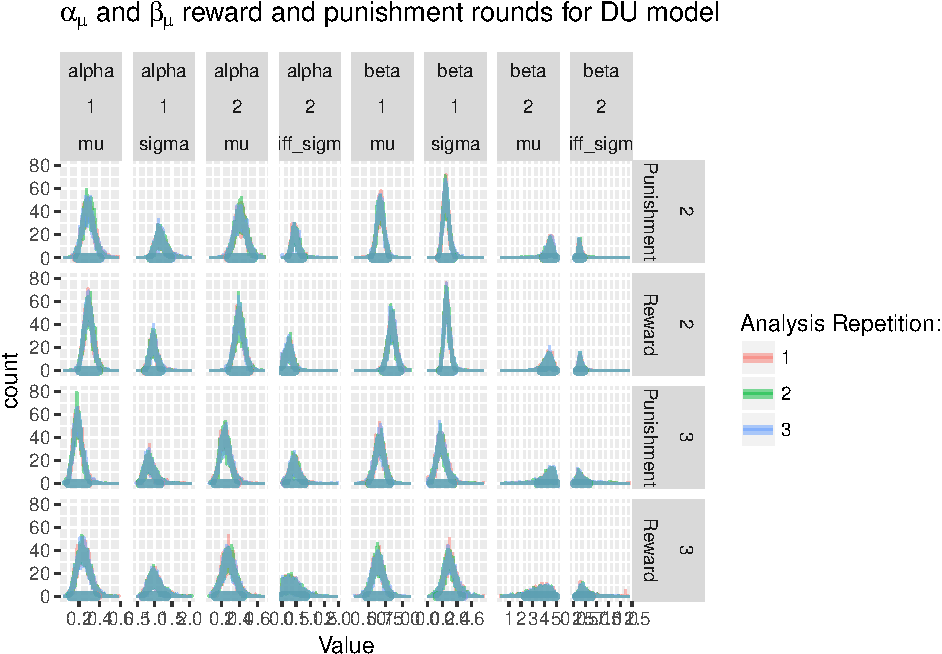
\includegraphics{compare_vb_and_MCMC_files/figure-latex/MCMCReliability-2.pdf}

MCMC seems to perform very consistently across runs. Thus, in subsequent
estimates there is no need to look at more than one Analysis Repetition.

\subsection{MCMC Representativness, accuracy, and
efficiency}\label{mcmc-representativness-accuracy-and-efficiency}

Considering the wide HDIs produced by our MCMC estimates, I want to take
a closer look to see if the MCMC estimates are representative, accurate,
and efficient. \footnote{cite Kruschke}

\subsubsection{Representativeness}\label{representativeness}

To assess Representativeness for an MCMC algorithm, we need to see
whether chains have converged such that initial randomly-chosen priors
are not related to final values. We can visually examine the trace plots
below, and we can, examine teh density plots, and examine the
Gelman-Rubin statistic (Gelman \& Rubin, 1992) or the ``potential scale
reduction factor'' or ``shrink factor''. In \(rstan\), this is available
as the statistic \(\widehat{r}\).

The figure above shows one representative trace plot for one model run.
Parameter estimates for all models looked stable like the ones shown
here.

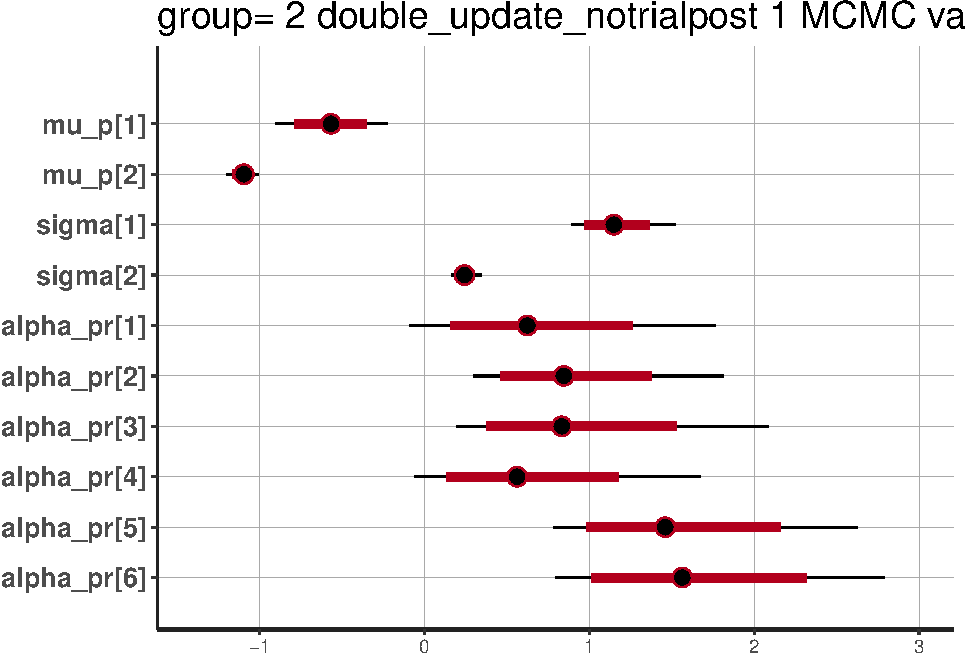
\includegraphics{compare_vb_and_MCMC_files/figure-latex/StanPlotLogResults-1.pdf}
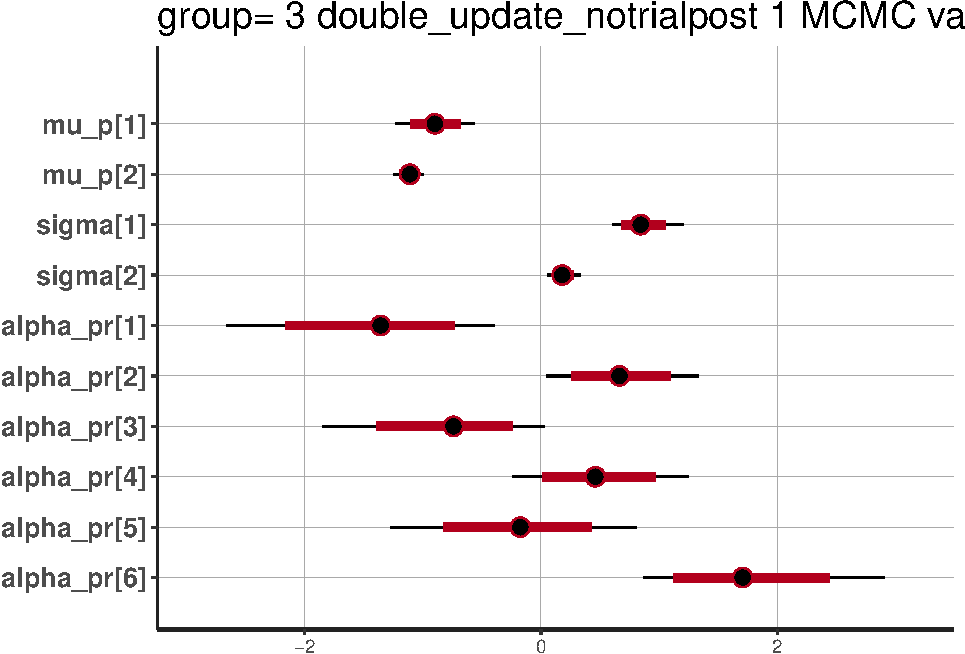
\includegraphics{compare_vb_and_MCMC_files/figure-latex/StanPlotLogResults-2.pdf}
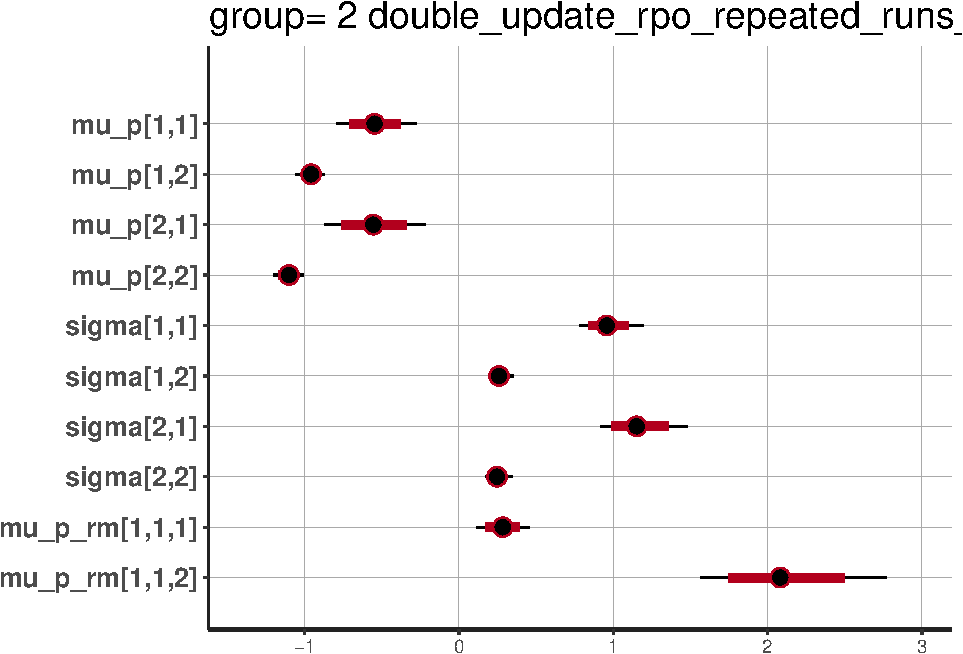
\includegraphics{compare_vb_and_MCMC_files/figure-latex/StanPlotLogResults-3.pdf}
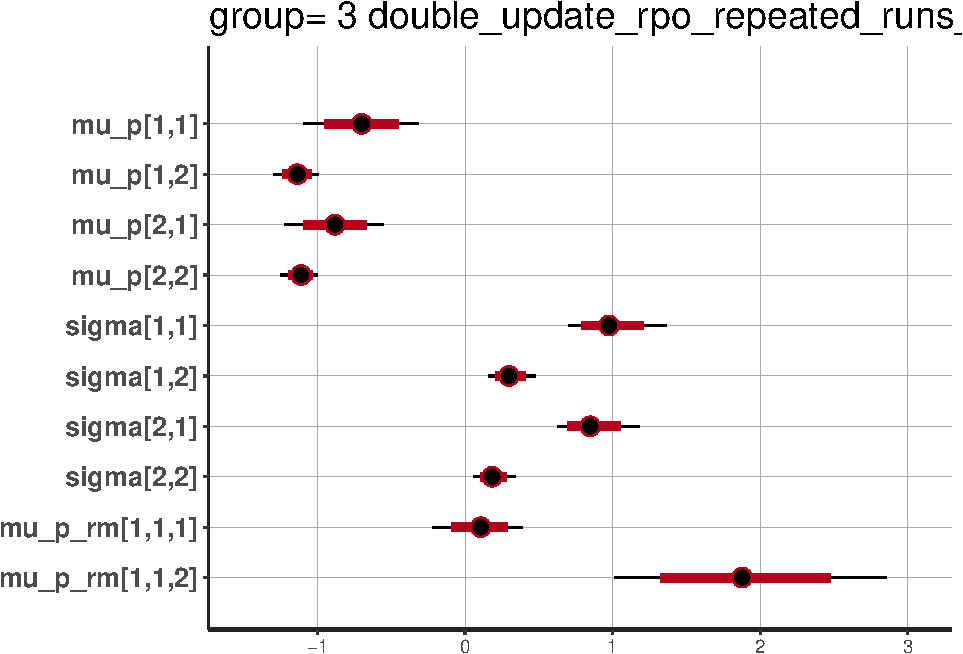
\includegraphics{compare_vb_and_MCMC_files/figure-latex/StanPlotLogResults-4.pdf}

Do we see overlap of the chains, or do they not overlap very much? Given
the traceplot, I'd expect high levels of overlap.

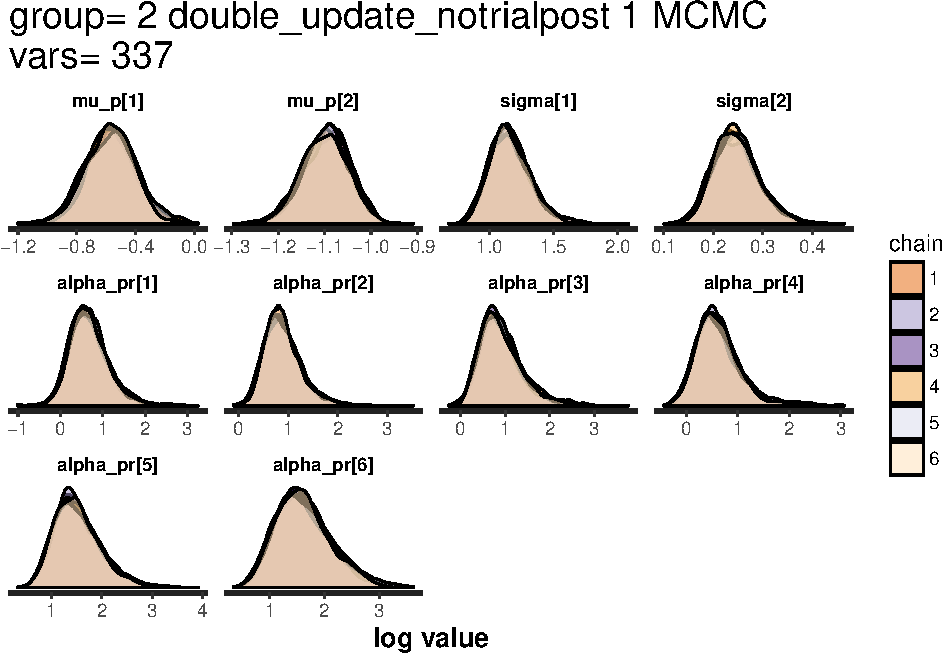
\includegraphics{compare_vb_and_MCMC_files/figure-latex/StanPlotDensity-1.pdf}
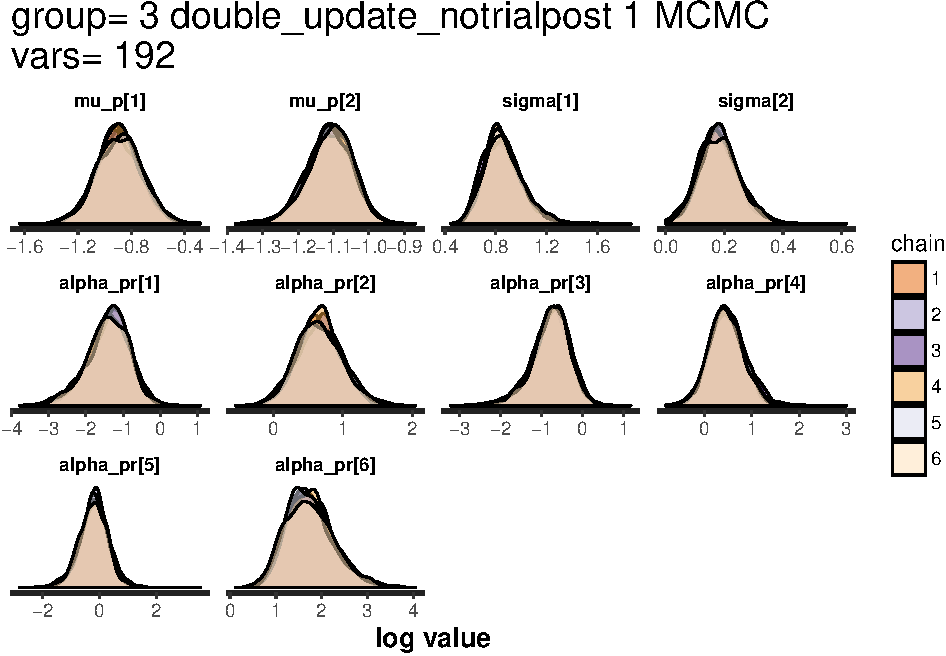
\includegraphics{compare_vb_and_MCMC_files/figure-latex/StanPlotDensity-2.pdf}
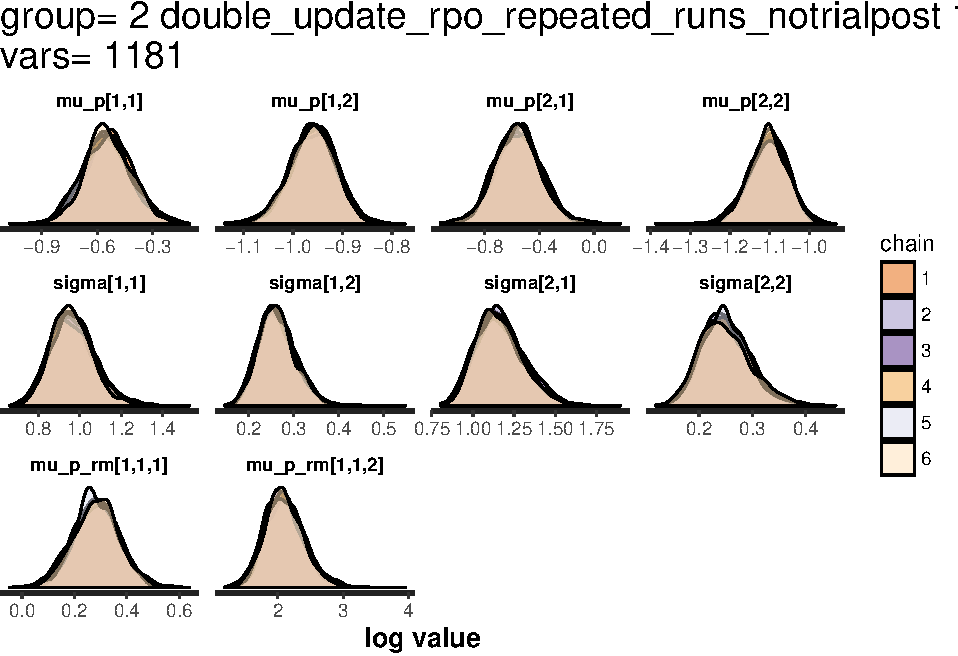
\includegraphics{compare_vb_and_MCMC_files/figure-latex/StanPlotDensity-3.pdf}
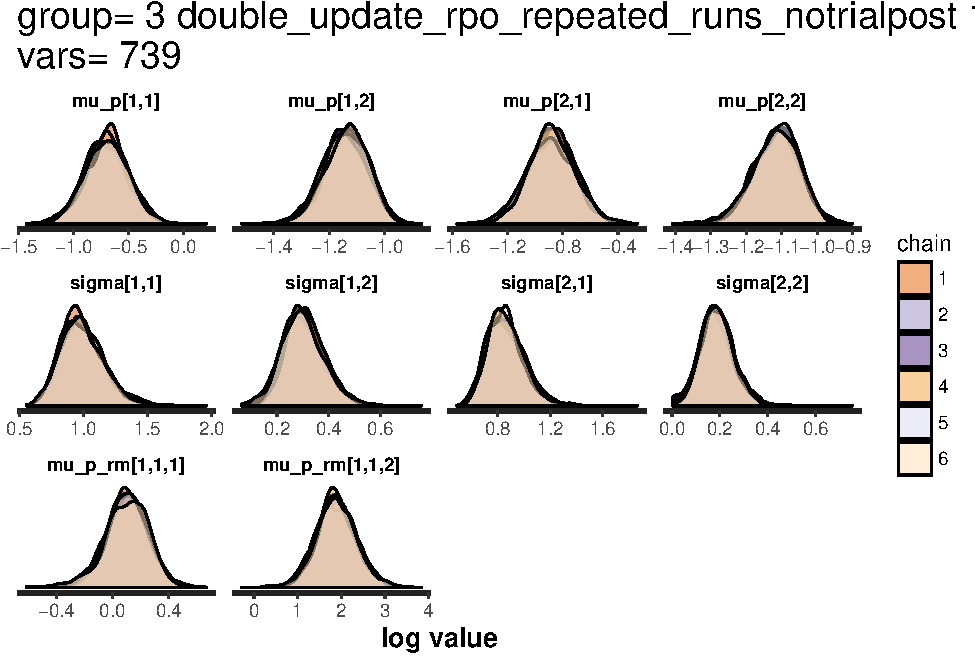
\includegraphics{compare_vb_and_MCMC_files/figure-latex/StanPlotDensity-4.pdf}

Visually, these seem pretty good, with the exception of Group 3, No
Trial Posteriors. As for MSCE and ESS\ldots{}

\begin{verbatim}
## Inference for Stan model: double_update_notrialpost.
## 6 chains, each with iter=2000; warmup=1000; thin=1; 
## post-warmup draws per chain=1000, total post-warmup draws=6000.
## 
##           mean se_mean   sd  2.5%   25%   50%   75% 97.5% n_eff Rhat
## mu_p[1]  -0.57       0 0.17 -0.90 -0.68 -0.57 -0.45 -0.22  1639    1
## mu_p[2]  -1.10       0 0.05 -1.20 -1.13 -1.10 -1.06 -1.00  2626    1
## sigma[1]  1.16       0 0.16  0.89  1.05  1.15  1.26  1.52  2999    1
## sigma[2]  0.25       0 0.05  0.16  0.21  0.24  0.27  0.35  1809    1
## 
## Samples were drawn using NUTS(diag_e) at Thu Oct  5 18:09:05 2017.
## For each parameter, n_eff is a crude measure of effective sample size,
## and Rhat is the potential scale reduction factor on split chains (at 
## convergence, Rhat=1).
## [1] "Increase in sample size required to get an ESS of 10^5 at this level of efficiency:"
##  mu_p[1]  mu_p[2] sigma[1] sigma[2] 
##      6.1      3.8      3.3      5.5 
## 
## 
## Inference for Stan model: double_update_notrialpost.
## 6 chains, each with iter=2000; warmup=1000; thin=1; 
## post-warmup draws per chain=1000, total post-warmup draws=6000.
## 
##           mean se_mean   sd  2.5%   25%   50%   75% 97.5% n_eff Rhat
## mu_p[1]  -0.89       0 0.17 -1.23 -1.00 -0.90 -0.78 -0.56  1779 1.00
## mu_p[2]  -1.11       0 0.07 -1.25 -1.15 -1.11 -1.07 -0.99  2664 1.00
## sigma[1]  0.86       0 0.15  0.60  0.75  0.84  0.95  1.20  2426 1.00
## sigma[2]  0.18       0 0.07  0.06  0.14  0.18  0.23  0.33  1517 1.01
## 
## Samples were drawn using NUTS(diag_e) at Thu Oct  5 18:16:08 2017.
## For each parameter, n_eff is a crude measure of effective sample size,
## and Rhat is the potential scale reduction factor on split chains (at 
## convergence, Rhat=1).
## [1] "Increase in sample size required to get an ESS of 10^5 at this level of efficiency:"
##  mu_p[1]  mu_p[2] sigma[1] sigma[2] 
##      5.6      3.8      4.1      6.6 
## 
## 
## Inference for Stan model: double_update_rpo_repeated_runs_notrialpost.
## 6 chains, each with iter=2000; warmup=1000; thin=1; 
## post-warmup draws per chain=1000, total post-warmup draws=6000.
## 
##             mean se_mean   sd  2.5%   25%   50%   75% 97.5% n_eff Rhat
## mu_p[1,1]  -0.54       0 0.13 -0.79 -0.63 -0.55 -0.46 -0.28  1552    1
## mu_p[1,2]  -0.96       0 0.05 -1.06 -0.99 -0.96 -0.93 -0.87  2259    1
## mu_p[2,1]  -0.55       0 0.17 -0.87 -0.67 -0.56 -0.45 -0.22  1186    1
## mu_p[2,2]  -1.10       0 0.05 -1.20 -1.14 -1.10 -1.07 -1.01  2365    1
## sigma[1,1]  0.97       0 0.11  0.78  0.89  0.96  1.03  1.20  2450    1
## sigma[1,2]  0.26       0 0.04  0.19  0.23  0.26  0.29  0.35  2310    1
## sigma[2,1]  1.17       0 0.14  0.92  1.06  1.15  1.25  1.48  2661    1
## sigma[2,2]  0.25       0 0.05  0.17  0.22  0.25  0.28  0.35  1904    1
## 
## Samples were drawn using NUTS(diag_e) at Thu Oct  5 20:11:15 2017.
## For each parameter, n_eff is a crude measure of effective sample size,
## and Rhat is the potential scale reduction factor on split chains (at 
## convergence, Rhat=1).
## [1] "Increase in sample size required to get an ESS of 10^5 at this level of efficiency:"
##  mu_p[1,1]  mu_p[1,2]  mu_p[2,1]  mu_p[2,2] sigma[1,1] sigma[1,2] 
##        6.4        4.4        8.4        4.2        4.1        4.3 
## sigma[2,1] sigma[2,2] 
##        3.8        5.3 
## 
## 
## Inference for Stan model: double_update_rpo_repeated_runs_notrialpost.
## 6 chains, each with iter=2000; warmup=1000; thin=1; 
## post-warmup draws per chain=1000, total post-warmup draws=6000.
## 
##             mean se_mean   sd  2.5%   25%   50%   75% 97.5% n_eff Rhat
## mu_p[1,1]  -0.70    0.01 0.20 -1.10 -0.83 -0.70 -0.57 -0.32  1190    1
## mu_p[1,2]  -1.14    0.00 0.08 -1.30 -1.19 -1.14 -1.08 -0.99  1662    1
## mu_p[2,1]  -0.88    0.00 0.17 -1.22 -0.99 -0.88 -0.77 -0.55  1944    1
## mu_p[2,2]  -1.12    0.00 0.07 -1.25 -1.16 -1.11 -1.07 -1.00  3318    1
## sigma[1,1]  0.99    0.00 0.17  0.70  0.87  0.97  1.10  1.37  2560    1
## sigma[1,2]  0.30    0.00 0.08  0.16  0.25  0.30  0.35  0.48  1128    1
## sigma[2,1]  0.86    0.00 0.14  0.63  0.76  0.85  0.95  1.18  2995    1
## sigma[2,2]  0.19    0.00 0.07  0.06  0.14  0.18  0.23  0.34  1305    1
## 
## Samples were drawn using NUTS(diag_e) at Thu Oct  5 21:18:58 2017.
## For each parameter, n_eff is a crude measure of effective sample size,
## and Rhat is the potential scale reduction factor on split chains (at 
## convergence, Rhat=1).
## [1] "Increase in sample size required to get an ESS of 10^5 at this level of efficiency:"
##  mu_p[1,1]  mu_p[1,2]  mu_p[2,1]  mu_p[2,2] sigma[1,1] sigma[1,2] 
##        8.4        6.0        5.1        3.0        3.9        8.9 
## sigma[2,1] sigma[2,2] 
##        3.3        7.7
\end{verbatim}

the Rhat values, which are Brooks-Gelman-Rubin statistics or ``potential
scale reduction factors'' (Broooks \& Gelman, 1998; Kruschke, 20xx)
should be close to 1--and definitely within 10\% of 1 (0.91 to 1.1). It
appears that one MCMC failed to converge but others converged
separately.

``\texttt{n\_eff}'' is the effective sample size. To get an effective
sample size of 10,000 for most parameters, we will need up to 887\% as
many post-warmup iterations as we currently have. Increasing chains form
6 to 12 will double the number of effective iterations, and an
additional increase by 443\% post-warmup iterations per chain, i.e.,
from 1000 to 4430, would enable us to reach 10,000. Adding an additional
10\% `buffer' to ensure we reach the target would bring us to 4873,
which we can round up to 5000.

\subsection{Accuracy}\label{accuracy}

To assess the \emph{accuracy} of the chains, we need to take into
account the \emph{effective sample size} (ESS)--how much independent
data actually exists in our analysis. To do this, we need a measure of
\emph{autocorrelation}. From ESS, we can get a measure of \emph{Monte
Carlo Standard Error}.

\subsubsection{Autocorrelation measures}\label{autocorrelation-measures}

We can view and measure autocorrelation in a number of ways: - To get
the effective sample size, we can use \texttt{rstan}'s
\texttt{stan\_ess}; bayesplot also offers
\href{\%5Bhttps://cran.r-project.org/web/packages/bayesplot/vignettes/visual-mcmc-diagnostics.html\#effective-sample-size}{appropriate
diagnostic tools}. Kruschke (20xx) recommends an effective sample size
of 10000 for estimating an HDI.

Kruschke advocates for an ESS of 10,000 for values like 95\% HDIs of
posteriors. Considering that we have 1000 post-warmup iterations and 6
chains, that equals 6000 iterations and ESS/SS appears to be in the
realm of 0.2-0.4. To get an ESS of 10,000, without optimizing the
function further, we'd need an actual sample size of 25,000 to 50,000.
Twelve chains of 4000 post-warmup iterations would get us 48,000, which
seems like a good amount to aim for.

\subsubsection{Monte Carlo Standard
Error}\label{monte-carlo-standard-error}

Monte Carlo Standard Error is calculated as

\[MCSE= ^{SD}/_{\sqrt{ESS}}\] or the standard formulation for standard
error, but with effective sample size used in place of actual sample
size.

We can view Monte Carlo Standard Error using the stan function
\texttt{stan\_mcse}.

\subsubsection{MCMC Efficiency}\label{mcmc-efficiency}

\emph{Efficiency} simply describes how efficient the estimation
algorithm is at calculating our model's result. This includes not only
measures like autocorrelation but also other model performance features
that could potentially slow it down.

Efficiency is one of Turner's key arguments for the use of DE-MCMC over
other forms of MCMC, such as the Metropolis-Hastings algorithm
(CITEREF:TURNER2013), or NUTS or Hamiltonian Markov Models (personal
communication) as implemented in Stan.

\subsection{Variational Bayes Representativness, accuracy, and
efficiency}\label{variational-bayes-representativness-accuracy-and-efficiency}

Do our diagnostic tools offer any insight into how we could improve
variationalBayes accuracy?

\subsubsection{Representativeness}\label{representativeness-1}

A trace plot isn't particularly informative; because there's only one
chain, we can't tell if there is convergence.

\begin{figure}[htbp]
\centering
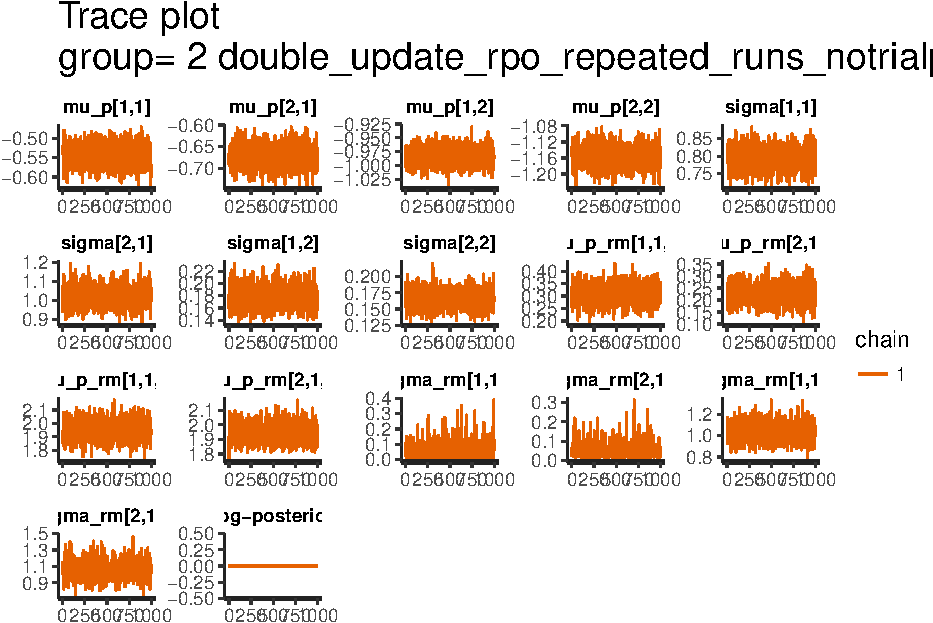
\includegraphics{compare_vb_and_MCMC_files/figure-latex/VBTraceplot-1.pdf}
\caption{TRUE}
\end{figure}

The trace plots does tell us that estimates seem to be stable, which
does suggest it's unlikely that we can improve performance by adding
additional iterations.

We don't really have the diagnostic tools available to diagnose
variationalbayes, although the stable trace plots make me think it's
unlikely we can get superior performance by adding iterations. Still,
with the low performance load of variational bayes, it won't hurt to
try.

\subsection{Model analysis}\label{model-analysis}

Does the model estimate common-sense parameter values?

I would hope to see that we get more variability across reward
vs.~punishment than across run1 vs.~run2.

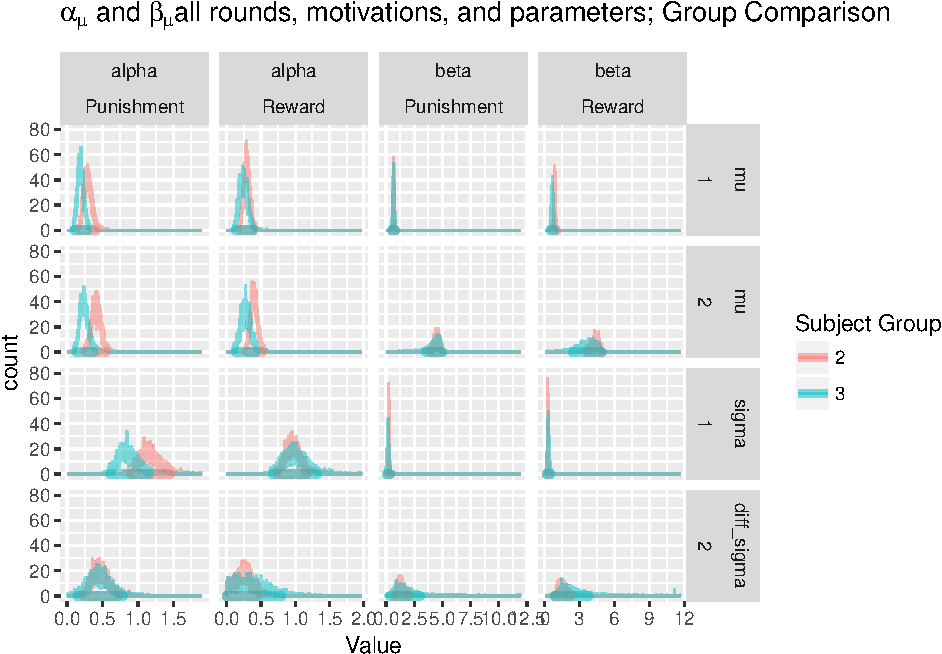
\includegraphics{compare_vb_and_MCMC_files/figure-latex/MCMCresultsGroupComparison-1.pdf}
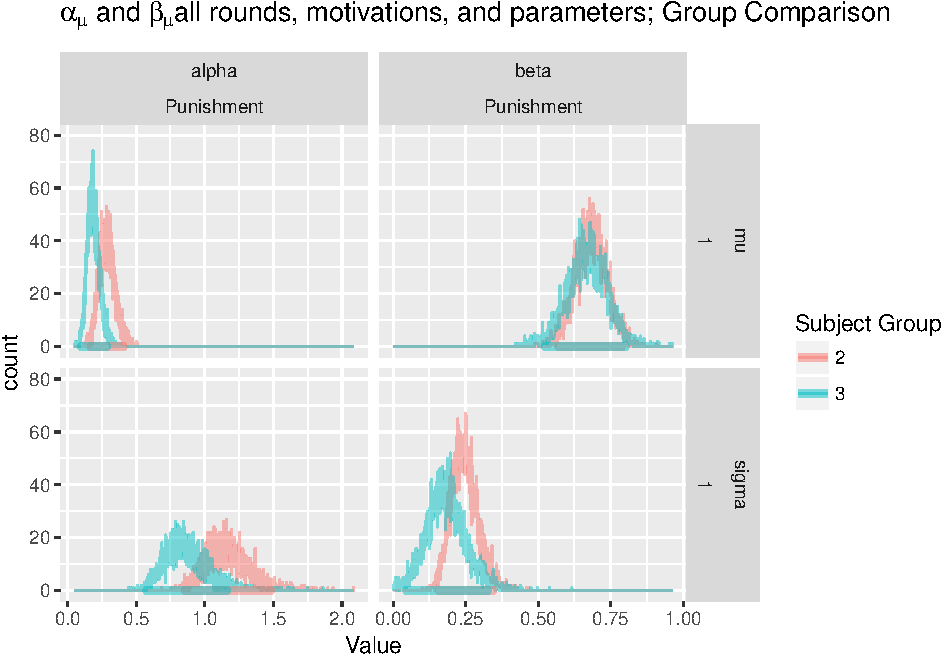
\includegraphics{compare_vb_and_MCMC_files/figure-latex/MCMCresultsGroupComparison-2.pdf}

\begin{figure}[htbp]
\centering
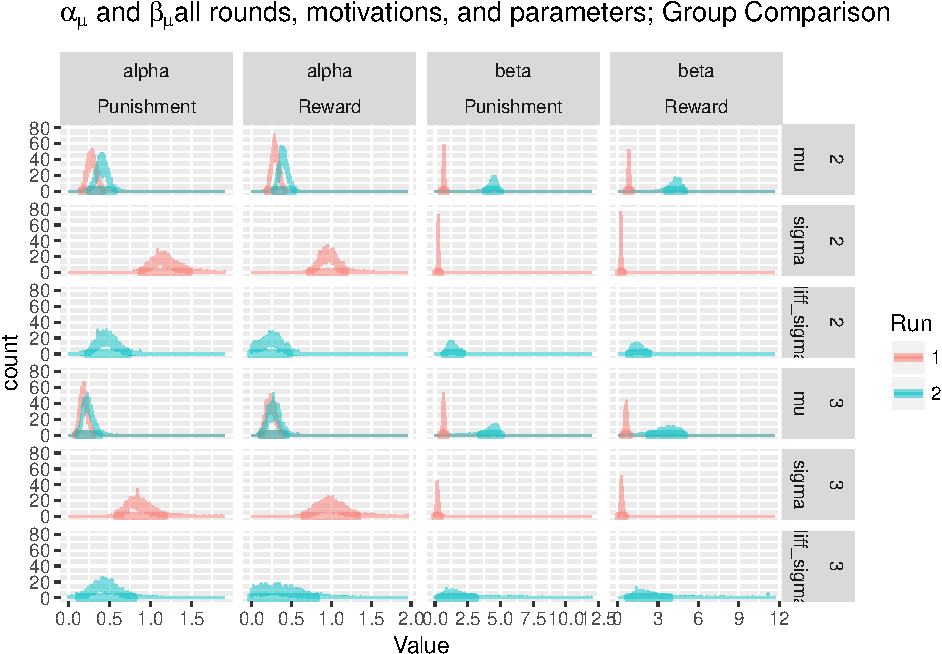
\includegraphics{compare_vb_and_MCMC_files/figure-latex/MCMCresultsRunComparison-1.pdf}
\caption{TRUE}
\end{figure}

\begin{figure}[htbp]
\centering
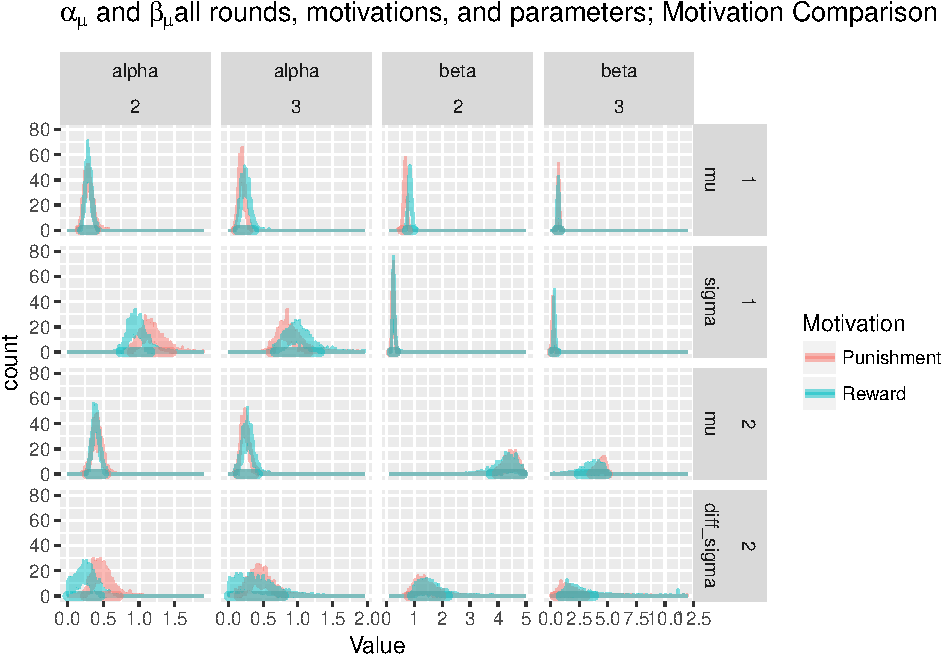
\includegraphics{compare_vb_and_MCMC_files/figure-latex/MCMCresultsMotivationComparison-1.pdf}
\caption{TRUE}
\end{figure}

There aren't clear differences between either reward and punishment,
between Group 2 and 3, or Run 1 and 2. It's not crazy data, but it is
disappointing and I want to see if we can do better.

\section{Discussion}\label{discussion}

We're going to try again. At the same time, because the trace plots have
seemed stable, it seems unlikely that adding iterations will change
anything. We'll see!


\end{document}
